\RequirePackage[l2tabu, orthodox]{nag}
\documentclass[a4paper,oneside,10pt]{article}

%include version control info
\input{vc.tex}

%\usepackage[bindingoffset=1.5cm,centering,includeheadfoot,margin=3cm]{geometry}

\usepackage[T1]{fontenc}
\usepackage[utf8]{inputenc}
\usepackage[pdftex]{graphicx}
%\usepackage{subfig}

\usepackage[protrusion=true,expansion=true]{microtype}

\usepackage{fancybox}
\usepackage{shadow}
\usepackage{xspace}
\usepackage{acronym}

%\usepackage{lmodern} % new latin extended computer modern font}, use with T1
%\usepackage{pxfonts} % has replaced palatino
\usepackage{cmbright}

\usepackage{listings}

\usepackage[allowlitunits]{siunitx}
% Try $20\micro\seconds$

%\addtolength{\oddsidemargin}{-1cm}
%\addtolength{\evensidemargin}{-1cm}
%\addtolength{\textwidth}{+2cm}
%\usepackage{showframe}
 
%\usepackage{lastpage}
% for \pageref{LastPage}

% fancy header
\usepackage{fancyhdr}
\pagestyle{fancy}
\fancyhf{} % clear default header and footer
\fancyhead[R]{\textit{\nouppercase{\leftmark}}}
\fancyhead[C]{}
\fancyfoot[R]{--\thepage--}
\fancyfoot[L]{Base revision~\GITAbrHash, \GITAuthorDate, \GITAuthorName.}

\setlength{\headheight}{14pt}

\newcommand\Hrule{\noindent\rule{\linewidth}{1.5pt}}
\newcommand{\sidenote}[1]{\marginpar{\scriptsize{\textsf{#1}}}} % Bram's sidenote for comments

%\usepackage{titlesec}

\usepackage[pdftex,
 pdfauthor={Matthias P. Braendli},
 pdftitle={ODR-mmbTools Documentation},
 pdfsubject={},
 pdfkeywords={Digital Audio Broadcasting,DAB,single-frequency network,SFN,mmbTools,ODR-mmbTools,open-source,software-defined radio},
 pdfcreator=pdflatex]{hyperref}
\hypersetup{colorlinks, citecolor=black, filecolor=black, linkcolor=black, urlcolor=black}

\newcommand{\weblink}[2]{\href{#1}{\url{#1}: \textsc{#2}}}
\newcommand{\us}{\,\si{\micro\second}\xspace}
\newcommand{\km}{\,\si{\kilo\meter}\xspace}
\newcommand{\ms}{\,ms}
\newcommand{\DABplus}{DAB$^\mathrm{+}$\xspace}
\newcommand{\captionwidth}{0.9\textwidth}
\newcommand{\mmbtools}{\mbox{ODR-mmbTools}}

% index stuff
\usepackage{tocbibind} % Index in TOC
%\usepackage{makeidx}
%\usepackage{showidx} % show index entries in margin
%\makeindex

%\newcommand{\bib}[4]{\item{\textsc{#1}, \emph{#2}, #3\\\hspace{2em}#4}}

% ---------------------------------------------------------

\newcommand{\titleinfo}{Documentation for the ODR-mmbTools
Open-Source Software-Defined \DABplus Tools}
\author{Matthias P. Brändli}
\date{2 May 2014}
\title{\titleinfo}


% Margins for handwritten notes
%\addtolength{\oddsidemargin}{-2cm}
%\addtolength{\evensidemargin}{-2cm}
%\addtolength{\textwidth}{-2cm}

\usepackage{color}
\definecolor{Brown}{cmyk}{0,0.81,1,0.60}
\definecolor{OliveGreen}{cmyk}{0.64,0,0.95,0.40}
\definecolor{CadetBlue}{cmyk}{0.62,0.57,0.23,0}
\definecolor{lightlightgray}{cmyk}{0,0,0,0.02}
\definecolor{gray}{cmyk}{0,0,0,0.8}

% LaTeX magic: make sections have a cleardoublepage
% Useful for twoside only
%\let\stdsection\section
%\renewcommand*\section{\cleardoublepage\stdsection}

\begin{document}
\lstset{
language=C,                             % Code langugage
basicstyle=\ttfamily,                   % Code font, Examples: \footnotesize, \ttfamily
keywordstyle=\color{OliveGreen},        % Keywords font ('*' = uppercase)
commentstyle=\color{gray},              % Comments font
numbers=left,                           % Line nums position
numberstyle=\tiny,                      % Line-numbers fonts
stepnumber=1,                           % Step between two line-numbers
numbersep=5pt,                          % How far are line-numbers from code
backgroundcolor=\color{lightlightgray}, % Choose background color
frame=none,                             % A frame around the code
tabsize=2,                              % Default tab size
captionpos=b,                           % Caption-position = bottom
breaklines=true,                        % Automatic line breaking?
breakatwhitespace=false,                % Automatic breaks only at whitespace?
showspaces=false,                       % Dont make spaces visible
showtabs=false,                         % Dont make tabls visible
morekeywords={uint32_t,uint8_t,uint16_t,time_spec_t,size_t,
clock_config_t},
}
\pagestyle{empty}
\pagenumbering{roman}
 \begin{titlepage}
    \null\vfil
    \begin{flushleft}
      \huge \textbf{\titleinfo}
    \end{flushleft}
    \par
    \hrule height 4pt
    \par
    \begin{flushright}
      \large
      \textsl{Project Documentation} \par
    \end{flushright}
    \vspace{\fill}
    \vspace*{\stretch{1}}

    \begin{center}
        \Large
        \textsc{Opendigitalradio\\\href{http://opendigitalradio.org}{http://opendigitalradio.org}\\2014}
    \end{center}
    \vspace{\fill}
    \vspace*{\stretch{2}}

    \begin{figure}[!h]
        \centering
        \parbox{1.2in}{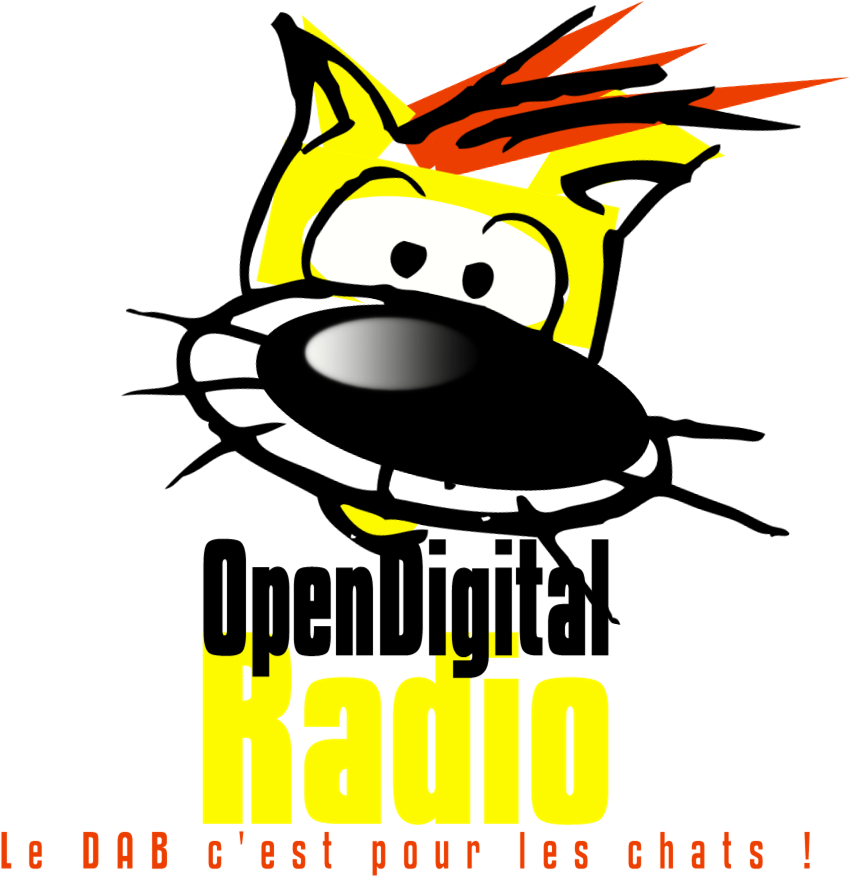
\includegraphics[width=10em]{figures/dab-pour-chats.jpg}}
        \qquad
    \end{figure}

    \vspace*{1cm}
 \end{titlepage}

\pagestyle{fancy}
\tableofcontents

\section*{Acronyms}
\markboth{Acronyms}{}
\addcontentsline{toc}{section}{Acronyms}
\begin{acronym}[mmbTools]
    \acro{1PPS}{One pulse per second}
    \acro{CIF}{Common Interleaved Frame}
    \acro{CRC}{Communications Research Centre Canada}
    \acro{DAB}{Digital Audio Broadcasting}
    \acro{DMB}{Digital Multimedia Broadcasting}
    \acro{ETI}{Ensemble Transport Interface}
    \acro{ETSI}{European Telecommunications Standards Institute}
    \acro{FIC}{Fast Information Channel}
    \acro{HE-AAC}{High Efficiency Advanced Audio Codec}
    \acro{mmbTools}{Mobile Multimedia Broadcasting Tools}
    \acro{MNSC}{Multiplex Network Signalling Channel}
    \acro{NTP}{Network Time Protocol}
    \acro{OCXO}{Oven-Controlled Crystal Oscillator}
    \acro{OFDM}{Orthogonal Frequency-Division Multiplexing}
    \acro{PRBS}{Pseudo-Random Bit Sequence}
    \acro{SFN}{Single-Frequency Network}
    \acro{TCXO}{Temperature-Compensated Crystal Oscillator}
    \acro{TIST}{Timestamp field in the ETI frame}
    \acro{TM}{Transmission Mode}
    \acro{UHD}{USRP Hardware Driver}
    \acro{USRP}{Universal Software-Radio Peripheral}
\end{acronym}

\pagenumbering{arabic}
% LICENSE: see LICENCE
\section{Introduction}
This is the official documentation for the \mmbtools. These tools can be used to
experiment with DAB modulation, learn the techniques behind it and setup a DAB
or \dabplus transmitter.

This documentation assumes that you are already familiar with base concepts of
the DAB system. To get started with the \mmbtools, understanding how the DAB
transmission chain is structured is a prerequisite. The ``DAB Bible'' by Hoeg
and Lauterbach~\cite{hoeg} and the ``Guide to DAB standards'' from the
ETSI~\cite{etsidabguide} can be used as a starting point.

In this document, the terms ``DAB'' and ``\dabplus'' are used somewhat
interchangeably, since many parts of the transmission chain are identical
between the two variants. In most cases, ``DAB'' will be used, and ``\dabplus''
when talking about specific details about the newer version of the standard.


\section{Purpose}
The different programs that are part of the \mmbtools each have their own
documentation regarding command-line options and configuration settings, and the
opendigitalradio.org wiki\footnoteurl{http://opendigitalradio.org}
contains many explanations and pointers, but there is
no single source of documentation available for the whole tool-set.

This document aims to solve this, by first outlining general concepts,
presenting different usage scenarios and detailing a complete transmission
setup.
With this document in hand, you should be able to understand all elements
composing a \mmbtools transmission chain, and how to set one up.

\section{Presentation of the Tools}
\subsection{Origins}
Before we begin with technical details, first a word about the history of
the mmbTools.
In 2002, Communications Research Centre Canada\footnoteurl{http://crc.ca}
started developing a DAB multiplexer. This effort evolved through the years, and
was published in September 2009 as \mbox{CRC-DabMux} under the GPL
open-source licence.

CRC also developed a DAB modulator, called \mbox{CRC-DABMOD}, which could create
baseband I/Q samples from an ETI file. This I/Q data could then be set to
a hardware device using another tool. For the Ettus USRPs, a ``wave player''
script was necessary to interface to GNURadio. Only DAB Transmission Mode 2 was
supported. \mbox{CRC-DABMOD} was also released under the GPL in early 2010.

As encoders, toolame could be used for DAB, and CRC developed a closed-source
\mbox{CRC-DABPLUS} \dabplus encoder.

These three CRC-~tools, and some additional services available on the now
unreachable website\footnote{There are some snapshots of the website available
    on \url{http://archive.org}.} \url{http://mmbtools.crc.ca} were
part of the \mbox{CRC-mmbTools}. These tools made it possible to set up the
first DAB transmission experiments.

In 2012, these tools received experimental support for single-frequency
networks, a functionality that has been developed by Matthias P. Brändli during
his Master's thesis\footnote{The corresponding report is available at
    \url{http://mpb.li/report.pdf}}.
Because SFNs are mainly used in TM 1, CRC subsequently released a patch to
\mbox{CRC-DABMOD} that enabled all four transmission modes.

At that point, involvement from CRC started to decline. The SFN patch was
finally never included in the \mbox{CRC-mmbTools}, and as time passed by, the
de-facto fork on \url{http://mpb.li} was receiving more and more features.
Having two different programs with the same name made things complicated, and
the tools were officially forked with the approval of CRC in February 2014, and
given the new name \mbox{ODR-mmbTools}. They are now developed by the
Opendigitalradio association.

In April 2014, the official \mbox{CRC-mmbTools} website went offline, and it has
become very difficult, if not impossible to acquire licences for the
\mbox{CRC-DABPLUS} encoder. Luckily there is an open-source replacement
available, which was part of Google's Android sources. This encoder has been
extended with the necessary \dabplus{}-specific requirements (960-transform,
error correction, framing, etc.), and now exists under the name
\mbox{fdk-aac}. The encoder \mbox{ODR-AudioEnc} can use this library to encoder
\dabplus{}.

\subsection{Included Tools}
The \mmbtools are composed of several software projects:
\mbox{ODR-DabMux}, \mbox{ODR-DabMod},
\mbox{ODR-AudioEnc}, \mbox{ODR-PadEnc}, and other scripts, bits and pieces
that are useful for the setup of a transmission chain.

\begin{figure}[h]
    \centering
    \smartdiagram[bubble diagram]{
        ODR-mmbTools,
        ODR-DabMux,
        ODR-DabMod,
        ODR-PadEnc,
        etisnoop,
        ODR-AudioEnc
    }
    \caption{The family of ODR-mmbTools}
    \label{fig:family_mmbTools}
\end{figure}

\subsubsection{ODR-DabMux}
ODR-DabMux implements a DAB multiplexer that combines all audio and data inputs
into an ETI output. It can be used off-line (i.e.~not real-time) to generate ETI
data for later processing, or in a real-time streaming scenario (e.g.~in a
transmitter).

It can read input audio or data from files (``.mp2'' for DAB, ``.dabp'' for
\dabplus), FIFOs (also called ``named pipes'') or a network connection. The
network connection can use UDP or ZeroMQ. The CURVE authentication mechanism
from ZeroMQ can also be used to authenticate the encoder, in order to avoid that
a third-party can disrupt or hijack a programme.

The ensemble configuration can be specified on the command line using the
options described in the manpage, or using a configuration file. The command
line options are kept to be compatible with CRC-DABMUX, but using the
configuration file is preferred, because it supports more options.


\subsubsection{ODR-DabMod}
ODR-DabMod is a software-defined DAB modulator that receives or reads ETI, and
generates modulated I/Q data usable for transmission.

This I/Q data which is encoded as complex floats (32bits per complex sample) can
be written to a file or pipe, or sent to a USRP device using the integrated UHD
output. Other SDR platforms can be used if they are able to accept the I/Q data.
The output of the modulator can also be used in GNURadio if format conversion or
graphical analysis (spectrum) is to be done.

\subsubsection{ODR-AudioEnc}
The ODR-AudioEnc encoder can be used to encode for DAB and \dabplus. It includes
a toolame-based MPEG encoder, and uses the \mbox{fdk-aac} library as an external
dependency to encode \dabplus{}.

The integrated TooLAME library is a MPEG-1 Layer II audio encoder that is used
to encode audio for the DAB standard. The original project has been unmaintained
since 2003, but the twolame fork that pursues the development removed the DAB
framing. Because of this, twolame is not suitable for DAB.

The necessary framing and error-correction that \dabplus{} mandates, the PAD
insertion, the ZeroMQ output and the ALSA input were then added by different
parties.

\subsubsection{ODR-PadEnc}
This encoder is able to generate programme associated data that can be injected
into ODR-AudioEnc. It supports DLS, reading from a file, and MOT Slideshow,
where the slides are read from a folder.

\subsubsection{etisnoop}
Etisnoop is not used in the broadcasting chain directly, but is an analysis tool
for ETI, described in the ETSI standard~\cite{etsidabeti}. ODR-DabMux can write
an ETI file that can be analysed with etisnoop. The tool can be used to verify
the multiplex signalling, the presence of data in the subchannels, and it can
decode audio into files.

Additionally, it can output statistics in YAML format, which is useful in
combination with an RTLSDR receiver and the \verb+dab2eti+ tool to monitor
transmissions.


% vim: spl=en spell tw=80 et

\appendix
% LICENSE: see LICENCE

\section{ODR-DabMux ETI file formats}
\label{etiformat}
ODR-DabMux supports three output formats for the ETI stream, that have been described on the mmbTools forum
website.\footnote{\url{http://mmbtools.crc.ca/component/option,com\_fireboard/Itemid,55/func,view/id,4/catid,13/\#28}}

The three formats are called \emph{framed}, \emph{streamed} and \emph{raw}.

The \emph{framed} format is used for saving a finite ETI stream into a file. Each frame does not contain any padding, and the
format can be described as follows:
\begin{lstlisting}
uint32_t nbFrames
// for each frame
  uint16_t frameSize
  uint8_t data[frameSize]
\end{lstlisting}

When streaming data, in which case the number of frames is not known in advance, the \emph{streamed} format can be used.
This format is identical to the first one except for the missing \texttt{nbFrames}.
\begin{lstlisting}
// for each frame
  uint16_t frameSize
  uint8_t data[frameSize]
\end{lstlisting}

The \emph{raw} format corresponds to ETI(NI), where each frame has a constant size of 6144 Bytes. The padding in this
case is necessary.
\begin{lstlisting}
// for each frame
  uint8_t data[6144]
\end{lstlisting}

In order to select the format, the following syntax for the \texttt{-O} option is used:
\texttt{-O file://filename?type=format}, where \texttt{format} is one of \verb+framed+, \verb+streamed+ or
\verb+raw+.


\section{Additional EDI TAGs used}
ODR defined and uses two additional EDI TAGs, whose content is described here.

ODR-AudioEnc inserts audio level metadata into the ``ODRa'' TAG. The TAG item is in the following format:
\begin{lstlisting}
  TAG Name="ODRa" [4 bytes]
  Length=4 [4 bytes]
  Left Audio Level [signed 16-bit integer]
  Right Audio Level [signed 16-bit integer]
\end{lstlisting}


The second EDI TAG ``ODRv'' contains version and uptime information for the EDI source.
\begin{lstlisting}
  TAG Name="ODRv" [4 bytes]
  Length=N+4 [4 bytes]
  Version [String of N bytes, UTF-8 encoded, not zero terminated]
  Uptime [unsigned 32-bit integer representing number of seconds since program start]
\end{lstlisting}


\section{Bibliography}
\bibliographystyle{acm}
\bibliography{dab}



\end{document}

% vim: spl=en spell tw=80 et
